\nonstopmode
\documentclass[11pt, a4paper]{article}
%\documentclass{IEEEtran}
\usepackage{booktabs}
\usepackage[utf8]{inputenc}
\usepackage[spanish]{babel}
\usepackage{float}

\usepackage{parskip} 
\usepackage{hyperref}

\usepackage[margin=2.9cm]{geometry}
\usepackage{array}
\usepackage{tabularx}
\usepackage{graphicx}
\usepackage{subcaption}
\usepackage{amsmath}
\graphicspath{{images/}}
\usepackage{adjustbox}
\usepackage{url}

\usepackage{minted}

\usepackage{svg}
\usepackage{svg-extract}
\usepackage{fancyhdr}

\usepackage{listings}

%manejo util de las referencias
\usepackage{etoolbox}
\patchcmd{\thebibliography}{\section*{\refname}}{}{}{}
\patchcmd{\thebibliography}{\addcontentsline{toc}{section}{\refname}}{}{}{}
%Declarando Variables globales
\newcommand{\typeofdoc}{Tesis}
\newcommand{\subject}{Moises}
\newcommand{\infname}{Diseño de un modelo por redes neuronales para la humedad
de suelo en un micro–invernadero} %Name of doc
\newcommand{\teacher}{Luis Barreto}
\newcommand{\startdate}{23 de septiembre 2021}

%Adicionales
\setlength{\headheight}{48pt}
\pagestyle{fancy}
\fancyhf{}
\lhead{
\includegraphics[height=1.5cm]{dZNbudei.jpg}}
\rhead{
\includegraphics[width=2.5cm]{logo-tecnm.png}}
\renewcommand*\contentsname{Índice}
%%codigo
\renewcommand{\lstlistingname}{Código} 
\usepackage{xcolor}

\definecolor{codegreen}{rgb}{0,0.6,0}
\definecolor{codegray}{rgb}{0.5,0.5,0.5}
\definecolor{codepurple}{rgb}{0.58,0,0.82}
\definecolor{backcolour}{rgb}{0.95,0.95,0.92}

\lstdefinestyle{mystyle}{
    backgroundcolor=\color{backcolour},   
    commentstyle=\color{codegreen},
    keywordstyle=\color{magenta},
    numberstyle=\tiny\color{codegray},
    stringstyle=\color{codepurple},
    basicstyle=\ttfamily\footnotesize,
    breakatwhitespace=false,         
    breaklines=true,                 
    captionpos=b,                    
    keepspaces=true,                 
    numbers=left,                    
    numbersep=5pt,                  
    showspaces=false,                
    showstringspaces=false,
    showtabs=false,                  
    tabsize=2
}
\lstset{style=mystyle}
%%%%%%%%%%%%%%%%%%%%%%%%%%%%%%%%%%%%%%%%%%%%%%%%%%%%%%%%%%%%%%%%%%%%%%%%%%%%%%%%%%%%%%%%%%%%%%%%%%%%
 
\begin{document}
\begin{titlepage}
    \centering
    \vfill
    
\includegraphics[width=0.6\textwidth]{dZNbudei.jpg}\par 
    \vfill
    {\scshape\LARGE \textbf{\typeofdoc}}\par\vspace{1cm}
    {\textbf{\infname}}\par
    {\subject}\par
    \par{Asesor a cargo: \teacher }
    \par\vspace{0.2cm}
    \vfill
    \begin{tabular}{l|c}
        Moisés Ezequiel Dominguéz Salcedo & 17170527 \\
    \end{tabular}
    \vfill
    {\startdate}
    \vfill
\end{titlepage}
\par\vspace{2mm}
\tableofcontents
\newpage
 
\section{Introducción}

Generalidades del modelado de sistemas


\section{Marco teórico} 
\subsection{Variables físicas involucradas en un micro-invernadero} 
\begin{enumerate}\itemsep=-0.5em
    \item Temperatura (fuera y dentro del invernadero).
    \item Humedad relativa (fuera y dentro del invernadero).
    \item Luz o radiación solar (fuera y dentro del invernadero).
    \item Ventilación.
    \item Humedad de suelo.
    \item Temperatura de suelo.
    \item Fecha y hora de las mediciones de cada variables.  
    \item Zona geográfica. 
\end{enumerate}
\subsubsection{Temperatura (fuera y dentro del invernadero)}
La temperatura es una magnitud física que indica la energía interna de un
cuerpo, o de un sistema termodinámico en general. Esta propiedad termodinámica
únicamente describe un estado macroscópico.
La temperatura se define como la medida de la energía cinética media de las
moléculas que la forman. Es decir, los movimientos de las partículas en su
interior.
Por otro lado, se puede definir según la mecánica estadística, como la derivada
de la energía respecto a la entropía a volumen constante.

\subsubsection{Humedad relativa (fuera y dentro del invernadero)}

La humedad es una variable física definida formalmente como la cantidad de agua
disuelta en un gas o absorbida en un sólido.  Es una variable importante en
muchos ámbitos; por ejemplo, en procesos de fabricación que deben ser
ejecutados respetando condiciones de humedad especificas para garantizar los
productos. A veces la clave está en la humedad del aire ambiental, y otras en
la humedad de los productos mismos. 
\subsubsection{Luz o radiación solar (fuera y dentro del invernadero)}

La radiación solar se puede considerar el factor ambiental más importante en
los cultivos bajo invernadero, pues influye en procesos relacionados con la
fotosíntesis, los balances de agua y energía, y el crecimiento y desarrollo del
cultivo. Por tal motivo, el manejo de la radiación solar en la producción bajo
invernadero es sin duda una de las actividades más importantes en la
Horticultura Protegida, dicha importancia se sustenta en la relación directa
que existe entre la producción de materia seca y rendimiento con la cantidad de
radiación interceptada por el cultivo. 

La radiación solar es la fuente de
energía utilizada por las plantas en el proceso de fotosíntesis, y la
eficiencia de su aprovechamiento por las plantas va a depender de la longitud
de onda que esta presenta.


En la actualidad existen varios tipos de cubiertas de plástico, mallas sombra y
pantallas, mediante las cuales es posible modificar la calidad y cantidad de
energía luminosa en los invernaderos, sin embargo, existen consideraciones para
lograr el mejor aprovechamiento de la radiación solar. 

\begin{enumerate}
    \item Los materiales usados como cubierta en los invernaderos, salvo
        excepciones, deben ser transparentes a las radiaciones luminosas para
        permitir el paso de la luz visible. 

    \item Todos los materiales empleados para cubiertas de invernaderos
        reflejan una fracción de la luz que reciben del sol, que va del 20 – 30
        \%, generalmente. Al diseñar un invernadero, debe evitarse la formación
        de zonas sombreadas de las mismas estructuras, al proyectar e incidir
        en el interior, siendo estas lo más delgadas posibles para evitar
        interrumpir el paso de la luz. 

    \item En la actualidad existen materiales para cubiertas que difunden la
        luz que pasa a través de ellos convirtiéndola en luz difusa, la cual
        tiene la particularidad de no emitir sombras y llegar a todas partes y
        en todas direcciones. 

    \item La cantidad de luz que penetra a los invernaderos depende de la
        orientación de los mismos y de la forma o diseño de la estructura, pero
        sobre todo del ángulo de la cubierta con respecto al sol. 

    \item Es recomendable que los materiales de cubierta de los invernaderos
        transmitan del 85 – 90 \% de la luz solar incidente.
\end{enumerate}

Extraído de
https://www.intagri.com/articulos/horticultura-protegida/importancia-de-la-radiacion-solar-en-la-produccion-bajo-invernadero
- Esta información es propiedad intelectual de INTAGRI S.C., Intagri se reserva
el derecho de su publicación y reproducción total o parcial.

\subsubsection{Ventilación}
El sistema de ventilación en un invernadero sustituirá el aire más caliente que
se encuentra en el interior por otra masa de aire más frío que procede del
exterior. De esta manera gran parte de la sobrecarga de calor puede evacuarse,
disminuyendo la temperatura y, a su vez, modificando la concentración de gases
y la humedad. Se puede adoptar dos sistemas de ventilación: ventilación
mecánica. y ventilación natural. El sistema de ventilación que se debe emplear
depende de las propiedades del edificio y del tipo de cultivo que se realice.

\begin{enumerate}
    \item Ventilación natural:

        En la ventilación natural, el aire caliente que se encuentra en el
        interior del invernadero asciende y sale al exterior por dos aperturas
        situada en la cubierta, mientras que la admisión se realiza desde dos
        aperturas en la parte baja de las fachadas laterales. De esta forma se
        crea un flujo de aire que abarca todo el recinto interior. Para este
        tipo de ventilación son necesarias grandes aberturas, entre un 15 \% y
        un 25 \% de la superficie de la cubierta, y no permite controlar la
        incidencia de la velocidad del aire sobre las plantas.
    \item Ventilación mecánica simple:

        La ventilación mecánica se basa en la renovación del aire instalando
        ventiladores electromecánicos en la cubierta o más parte alta de una
        fachada lateral del invernadero, mientras que las entradas de aire que
       proviene del exterior se localizan en la parte baja de la pared
        opuesta.  Con este sistema la temperatura mínima interior no suele
        exceder de la del aire exterior.  

\end{enumerate}
\subsubsection{Humedad de suelo}
Unos niveles suficientes de humedad del suelo son una condición importante para
la formación adecuada de las plantas y el alto rendimiento de los cultivos.
Para la planta, el agua no sólo sirve como agente de restauración de la
humedad, sino también como regulador de la temperatura. En el proceso de
termorregulación, la planta evapora hasta el 99\% del agua obtenida, utilizando
sólo entre el 0,2\% y el 0,5\% para la formación de la masa vegetativa. Por lo
tanto, es fácil comprender que la planta tiene diferentes necesidades de
humedad según las condiciones climáticas y las etapas de crecimiento.
\subsubsection{Temperatura de suelo}
La temperatura es una propiedad que posee un efecto muy importante sobre los
organismos y sobre los procesos de alteración química de la fracción mineral
del suelo. Cada especie cultivada posee un rango propio de aptitud para la
germinación de la semilla, por ejemplo.  

La mayor parte de la energía calorífica que recibe el suelo procede de la
energía solar. En un clima templado, y por término medio, se estima que el
suelo recibe 144 calorías $día^{-1}* cm^{-2}$.  Obviamente, este valor varía con la
latitud, la época del año, la nubosidad, la orientación de la ladera y la
cubierta vegetal. 

La temperatura del suelo depende del balance de energía térmica absorbida,
emitida y reflejada \ref{fig:temperaturasuelo} Por lo tanto, la capacidad del suelo para
elevar su temperatura dependerá de una serie de variables intrínsecas (color,
humedad, calor específico, drenaje, renovación de la atmósfera del suelo, etc.)
y extrínsecas (humedad atmosférica, nubosidad, partículas en suspensión en la
atmósfera, precipitación, viento, relieve, vegetación, etc.). De manera más
detallada, los principales factores que influyen sobre la absorción de energía
solar por el suelo, son los siguientes: 

\begin{enumerate}
    \item El ángulo de incidencia de los rayos solares. La temperatura
        alcanzada es mayor cuando los rayos inciden de manera perpendicular al
        suelo. Este factor varía con la latitud (la temperatura alcanzada es
        mayor en el ecuador y disminuye cuando nos acercamos a los polos;
        ), la estación (los rayos solares en nuestras latitudes
        llegan con mayor inclinación en invierno que en verano) y
        el momento del día (la máxima perpendicularidad se alcanza al mediodía)
        . También como consecuencia de la orientación del sol, en
        nuestra latitud, las laderas orientadas al sur reciben más insolación
        que las orientadas al norte.  
    \item Las nubes atenúan la intensidad de
        la radiación solar. Sin embargo, pueden emitir radiación infrarroja, lo
        que es perceptible durante la noche.  La nubosidad minimiza la
        oscilación térmica entre el día y la noche.  
    \item Los suelos de color
        oscuro absorben mayor cantidad de energía térmica que los de color
        claro.  
    \item La humedad del suelo puede regular la temperatura, ya que
        el agua es un conductor del calor más rápido que la tierra, pero posee
        una gran inercia térmica. Por esta razón, los suelos más húmedos se
        calientan y enfrían más lentamente que un suelo seco. Por otra parte,
        la evaporación contribuye al mantenimiento de una temperatura más
        fresca.   
    \item La conductividad térmica del aire es muy
        baja. Por esta razón, los horizontes superficiales, si están bien
        aireados, difunden mal el calor hacia los horizontes inferiores, de
        modo que el suelo se calienta y enfría más rápidamente que un suelo
        poco poroso.  
    \item La vegetación y los restos de hojarasca (la capa de
        residuos vegetales del suelo se denomina frecuentemente como mulch)
        proporcionan una sombra que reduce el calentamiento del suelo durante
        el día. Además, pueden actuar como un aislante que evita la pérdida de
        energía térmica durante la noche.  En nuestras latitudes, la superficie
        de los suelos desprovistos de vegetación puede alcanzar los 40ºC en
        verano, con lo que se detiene la actividad biológica y se frenan los
        procesos edafogénicos.  
\end{enumerate}
\begin{figure}[H]
    \centering
    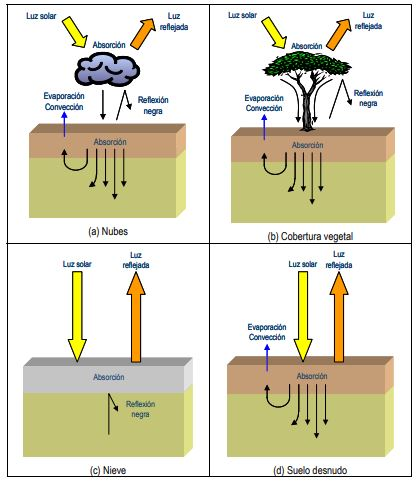
\includegraphics[width=\textwidth, keepaspectratio,
    heigh=7cm]{images/temperaturasuelo.JPG}
    \caption{Comportamiento de la temperatura en funciones de los distintos
    parámetros listados. }
    \label{fig:temperaturasuelo}
\end{figure}

\subsubsection{Localización}

Para determinar la zona donde estará ubicado el invernadero se
consideran los siguientes parámetros.

\begin{enumerate}
    \item Sanidad del terreno.

        Verificar que el terreno esté en excelentes condiciones e indagar sobre
        su historial. En el caso de siembras de tomate, evitar en lo posible
        sembrar en terreno donde anteriormente se hayan cultivado especies como
        pimiento o berenjena entre otros, los cuales pertenecen a la familia
        botánica del tomate (solanáceas), cuyas plagas y enfermedades
        generalmente son las mismas. Así mismo, evitar terrenos que
        anteriormente hayan sido usados como basureros o en otras actividades
        que puedan haber causado contaminación al suelo
    \item Fertilidad del terreno. 

        Se debe realizar un análisis del suelo para evaluar sus condiciones
        físicas y su composición química y microbiológica, que permita
        determinar si reúne las condiciones adecuadas para el desarrollo del
        cultivo.
    \item Drenaje del terreno. 

        Se debe seleccionar el mejor suelo con un buen drenaje y fertilidad. Un
        alto nivel freático puede limitar considerablemente la producción de
        tomate, principalmente por el ataque de enfermedades.
    \item Disponibilidad y calidad de agua de riego. 

        El invernadero debe estar cerca a fuentes de agua de excelente calidad,
        libre de contaminantes químicos y microbiológicos; debe existir un
        tanque de reserva para emergencias o épocas de sequía. El productor
        debe prever la cantidad de agua que será necesaria durante el
        desarrollo del cultivo, así como tener en cuenta los medios para su
        conducción y distribución.
    \item Historial de la información climática de la zona.

        En lo posible tener información acerca del comportamiento climático de
        la región: temperaturas máximas y mínimas tanto diurnas como nocturnas,
        comportamiento de la humedad relativa en la madrugada y en las horas de
        la tarde, velocidad y dirección del viento, horas y cantidad de los
        niveles de radiación, cantidad anual y máximo de mm/hora de las
        lluvias, y presencia de heladas, granizo y fenómenos naturales.

    \item Adecuada ventilación. 
    
        Se debe ubicar el invernadero en zonas donde exista suficiente
        ventilación para favorecer la remoción del aire húmedo o caliente desde
        su interior y de esta manera evitar la alta o baja humedad relativa que
        favorece el desarrollo de enfermedades, plagas, desórdenes fisiológicos
        y problemas de calidad y productividad en la planta. Cuando predominan
        vientos demasiado fuertes, también se producen condiciones
        desfavorables para el desarrollo de las plantas, especialmente
        condiciones de humedad relativa baja, por lo tanto será necesaria la
        ubicación de barreras vivas para disminuir la velocidad del viento.
    \item Luminosidad. 

        Se debe evitar ubicarlo cerca de árboles altos, construcciones o
        barreras geográficas como montañas que impidan la entrada de luz al
        invernadero.
    \item Pendiente del terreno. 

        Lo ideal es ubicar el invernadero en zonas de topografía plana
        adecuando el drenaje del terreno, pero si el terreno presenta alguna
        pendiente ésta no debe superar el 20%.
    \item Orientación. 

        Es importante ubicar el invernadero en sentido norte sur o de acuerdo a
        los ángulos de radiación para lograr la máxima penetración de la luz y
        minimizar el sombrío de las plantas a lo largo del día.
    \item Calidad de la estructura. 

        Lo ideal es construir un invernadero con materiales duraderos, como el
        acero galvanizado; en caso de utilizar madera o guadua se recomienda
        que éstas sean sometidas a algún tratamiento de inmunización para
        incrementar su vida útil.

\end{enumerate}


\subsection{Monitor de sensores}


\subsubsection{MQTT broker}
MQTT( MQ telemetru transport) es un protocolo de mensajería comúnmentete
utilizado en sistema o dispositivos IoT, basado en el patron
publish/subscribe, donde los mensajes son publicados en un tópico de un MQTT
broker que se encarga de distribuirlos a todos sus subscriptores que se hayan
subscrito al tópico . 
\begin{figure}[H]
    \centering
    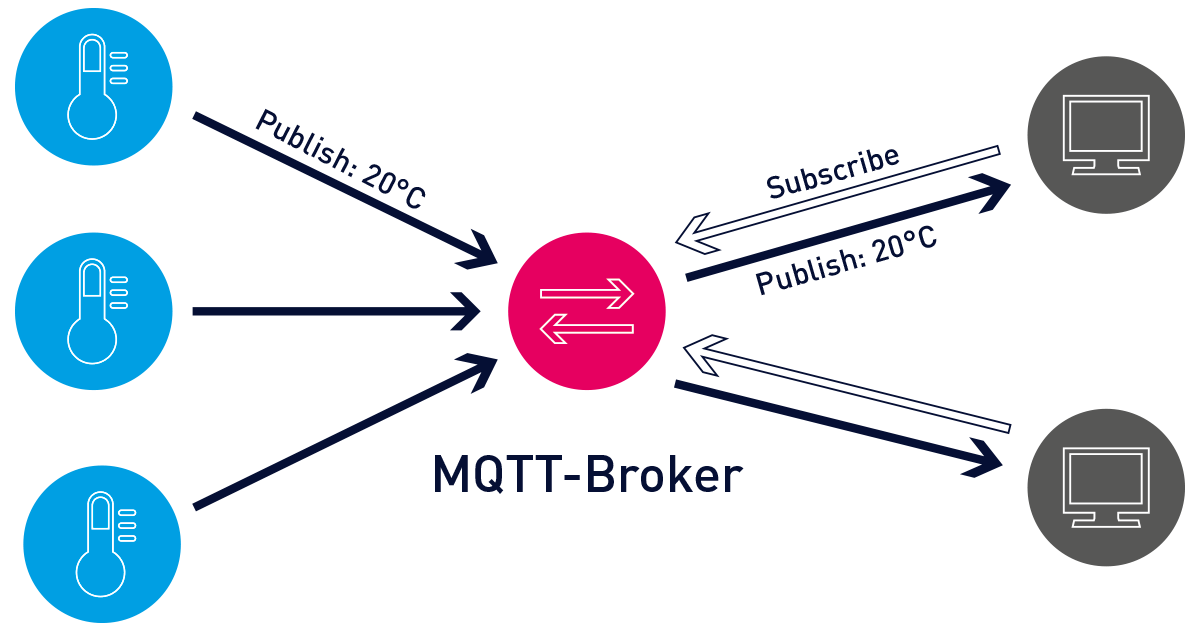
\includegraphics[width=\textwidth, keepaspectratio,
    height=7cm]{images/mqtt-architecture.png}
    \caption{Arquitectura de un broker MQTT}
    \label{fig:mqtt_arquitecture}
\end{figure}

Para la estación de monitoreo se esta haciendo uso de un borker  MQTT de codigo
abiero llamado \href{http://mosquitto.org}{eclipse mosquito}.

\subsubsection{Telegraf}
Telegraf es un agente que nos permite recopilar y reportar métricas. Las
métricas recogidas se pueden enviar a almacenes de datos, colas de mensajes o
servicios como: InfluxDB, Graphite, OpenTSDB, Datadog, Kafka, MQTT, NSQ, entre
otros.

\begin{figure}[H]
    \centering
    
\includegraphics[width=\textwidth, keepaspectratio,
    height=5cm]{images/logo-telegraf-1.jpg}
    \caption{telegraf}
    \label{fig:logo_telegraf}
\end{figure}

\subsubsection{InfluxDB}
Es un sistema gestor de bases de datos diseñado para almacenar bases
de datos de series temporales (TSBD - Time Series Databases). Estas bases de
datos se suelen utilizar en aplicaciones de monitorización, donde es necesario
almacenar y analizar grandes cantidades de datos con marcas de tiempo, como
pueden ser datos de uso de cpu, uso memoria, datos de sensores de IoT, etc.

\begin{figure}[H]
    \centering
    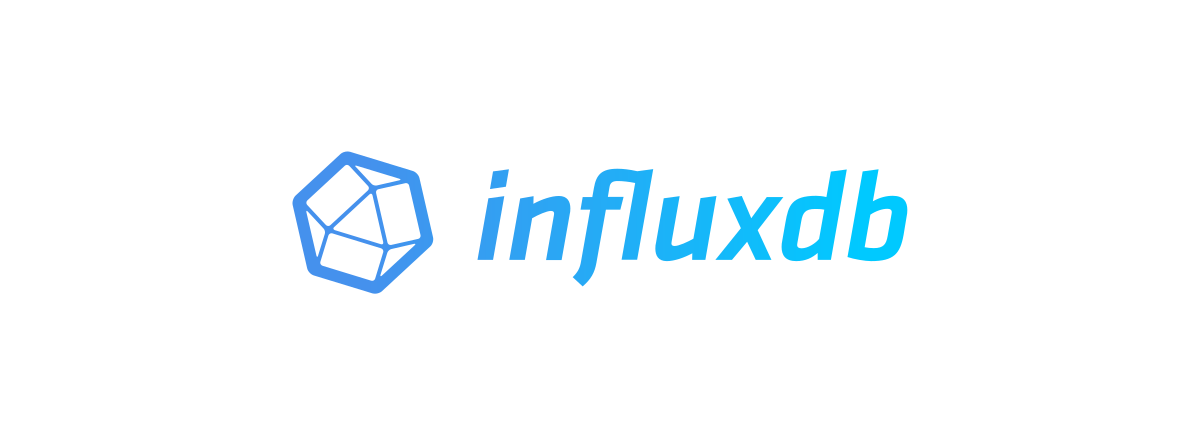
\includegraphics[width=\textwidth, keepaspectratio,
    height=5cm]{images/Influxdb_logo.svg_.png}
    \caption{Influxdb}
    \label{fig:logo_influx}
\end{figure}
\subsubsection{Grafana}
Es un servicio web que que permite visualizar en un panel de control
los datos almacenados en InfluxDB y otros sistemas gestores de bases de datos
de series temporales.
\begin{figure}[H]
    \centering
    
\includegraphics[width=\textwidth, keepaspectratio,
    height=5cm]{images/1200px-Grafana_logo.svg.png}
    \caption{Grafana}
    \label{fig:grafana}
\end{figure}




\subsection{Topologías empleadas en el modelado de sistemas}
\subsubsection{Modelado convencional}

\subsubsection{Redes neuronales empleadas como métodos alternativos}
Las redes neuronales artificiales ´(ANN) simulan al  sistema nervioso, que
aprende y reacciona frente a estímulos externos. Son agrupaciones de neuronas
unidas por enlaces que transmiten información a otras neuronas, las cuales la
transforman mediante una función de  excitación. \par Las ANN aprenden de la
información histórica a través de un entrenamiento o ajuste de los parámetros
de la red, que procesa los estímulos y entrega la respuesta deseada,
adquiriendo la capacidad de predecir nuevos estados del mismo fenómeno. Las
redes neuronales pueden tener diversas configuraciones.El número de capas
ocultas, así como el número de neuronas en cada una de las capas puede variar
según las necesidades del problema a resolver. \cite{brahm2003disminucion}

\section{Planteamiento del problema} 
El problema inicial
\section{Antecedentes}

\textbf{Redes neuronales para modelar predicción de heladas}
\cite{ovando2005redes} 
\par En este trabajo se desarrollaron modelos basados en redes neuronales del
tipo "backpropagation", para predecir la ocurrencia de heladas, a partir de
datos meteorológicos de temperatura, humedad relativa, nubosidad, dirección y
velocidad del viento. El entrenamiento y la validación de las redes se
realizaron utilizando 24 años de datos meteorológicos correspondientes a la
estación de Río Cuarto, Córdoba, Argentina, separados en 10 años como conjunto
de datos de entrenamiento y 14 como conjunto de datos de validación. Se
construyeron diferentes modelos para evaluar el comportamiento de las redes
cuando se usan distintos números de variables de entrada y/o neuronas en la
capa oculta y las probabilidades de aciertos en los resultados de predicción
para los mismos, al considerar distintas variables de entrada. En los modelos
realizados, el porcentaje de días con error de pronóstico fue de 2\%,
aproximadamente, para 14 años de aplicación; cuando se consideran días de
heladas efectivas no pronosticadas los porcentajes oscilan entre un 10\% y un
23\%, para el mismo período. Los resultados de la simulación muestran el buen
desempeño y la pertinencia general de esta metodología en la estimación de
fenómenos de comportamiento no lineal como las heladas.

\par\textbf{Diseño de un control electrónico automático para la concentración
de dióxido de carbono en un microclima de jitomate fundamentado en un sistema
dinámico}
\cite{ponce2015diseno} 
\par En el presente trabajo de tesis se consideran los modelos dinámicos del
cultivo de jitomate y del microclima, con la finalidad de obtener una ley de
control óptima que permita conocer el comportamiento óptimo de todas las
variables involucradas en el sistema conjunto microclima-cultivo, y así,
diseñar el dispositivo electrónico que controlará la concentración de dióxido
de carbono en microclimas de jitomate.  \par El modelo dinámico conjunto
microclima-cultivo está formado por las variables de estado involucradas en
ambos sistemas, estas variables son: biomasa de frutos, biomasa de
hojas,consumo de nutrientes y concentración de dióxido de carbono. A partir de
la teoría de control óptimo y del sistema conjunto se selecciona una función de
costos, la cual tiene la finalidad de minimizar el gasto por consumo de energía
y maximizar la producción total de jitomate, después se obtiene un sistema de
variables adjuntas que permite evaluar al sistema en las condiciones finales
deseadas. Este procedimiento proporciona una ley de control que deberá depender
de una o más variables.  Después se resuelve el sistema de variables de estado
junto con el sistema de variables adjuntas y el resultado es el comportamiento
óptimo de todas las variables. Se hace el estudio de dicho comportamiento, en
especial, el de la variable de estado de concentración de CO2, ya que, este
comportamiento será la señal de referencia que deberá seguir el sistema de
control electrónico.

\par\textbf{Un procedimiento efectivo para descomponer y modelar series
temporales en agricultura} 
\cite{aragon2018procedimiento} 
\par En este trabajo proponemos una forma innovadora de abordar casos reales de
predicción de la producción de cultivos en una cooperativa. Nuestro enfoque
consiste en la descomposición de la serie temporal original de los cultivos en
sub-series temporales según una serie de factores, con el objetivo de generar
un modelo predictivo del cultivo a partir de los modelos predictivos parciales
de las sub-series. El ajuste de los modelos se realiza mediante un conjunto de
técnicas estadísticas y de Aprendizaje Automático. Esta metodología se ha
comparado con una metodología intuitiva que consiste en una predicción directa
de las series temporales. Los resultados muestran que nuestro enfoque logra un
mejor rendimiento de predicción que la manera directa, por lo que aplicar una
metodología de descomposición es mas adecuada para este problema que la no
descomposición.

\par\textbf{Aplicación de técnicas de aprendizaje automático para la
agricultura altoandina de Perú} 
\cite{caceresaplicacion}
\par En este trabajo se presentan  y describen las técnicas utilizadas en el
campo del aprendizaje automático. 


\section{Hipótesis}
Durante el tratamiento del trabajo, dentro de los requerimientos es necesario
analizar y definir los posibles casos que se pueden presentar en el modelado
por redes neuronales. 

    
En la investigación se definen las las siguientes hipótesis. 
\begin{itemize}
    \item {Las variables físicas involucradas en el micro-invernadero,
        describen de manera acertada los fenómenos físicos involucrados dentro
        de este, las variables mencionadas corresponde a humedad, temperatura,
    medidas por un sensor de tipo THD-D producido por Autonics.}
    \item {Mediante el estudio y monitoreo de las variables físicas
           involucradas se determina la variable con mayor efecto sobre las
           condiciones físicas a las que se pudiese encontrar sometida la humedad de
           suelo.}
    \item {Las humedad de suelo esta relacionada estrechamente con las
        condiciones en el aire, tipo suelo, temporada del año, y zona
    geográfica.  dentro del habitáculo(invernader).}
\item {Implementar un sistema de monitoreo de los distintos sensores y
    actuadores involucrados.}
\end{itemize}
\section{Objetivo}
Diseñar un modelo empleando sistemas de aprendizaje autónomo, aprendizaje de
maquinas, para la humedad de suelo en un micro-invernadero.
\subsection{Objetivos específicos}
\begin{enumerate}
    \item {Ampliar el campo de estudio en las áreas de modelado y control, con
        un enfoque en la tecnologías en tendencias.}
    \item {Desarrollo de un modelo un modelo   inteligente utilizando
        herramientas del campo del aprendizaje autónomo}
    \item Describir el comportamiento de humedad de suelo en un
        micro-invernadero. 
\end{enumerate}
\section{Justificación}
Los modelos que describen las dinámicas de un sistema como en el casos de los
siguientes tipos de sistemas Los modelos que describen la dinámica de un
sistema como en el caso de los invernaderos, son de suma importancia para el
estudio de distintos métodos de control. Comúnmente los modelos son
representaciones matemáticas de los sistemas físicos normalmente un modelo se
utiliza para describir dinámicas de diferentes tipos de sistemas. Estos pueden
ser sistemas complejos y generalmente se busca obtener el modelo que represente
un ambiente de trabajo de la forma más óptima y eficiente que sea posible.
Durante el periodo ene-junio 2021 en el laboratorio de mecatrónica y control de
posgrado en el tecnológico de Culiacán, se realizó la documentación relacionada
al modelado matemático de estos sistemas.



\par Se destacan alguna característica, tales como un sistema multi-entrada
(sistemas tipo mimo), para controlar múltiples salidas.  Dada la complejidad de
estos sistemas se busca emplear una alternativa, como los sistemas de
aprendizaje automático, criterios de redes neuronales, buscando una solución
que se basa en datos reales del sistema que se desea describir para representar
un sistema no-lineal (sistema invernadero).  

\par Por lo tanto, en este trabajo se desarrollará un modelo basado en una
estructura de redes neuronales para determinar el comportamiento de la humedad
de suelo en un micro – invernadero.

\subsection{Referentes mexicanos}
%\begin{itemize}
    \item DR. Raul rojas Universidad de berlin.\par 
    La inteligencia artificial es el desarrollo de computadoras, que peudan emular alguna capacidad o inteligencia de un ser vivo o humano.
    \item Dr. humberto Sossa CIC-IPN\par
    Una maquina inteligente es capz de tomar decisiones apropiadas en circuistancias inciertas y ademas aprender de sus experiencias para reducir errores. 
\end{itemize} 
\section{Limitantes}
\subsection{Limitaciones en el campo de modelado con redes neuronales}
Las redes neuronales artificiales (ANN) tienen un problema para modelar los
fenómenos de lluvia y escorrentía: el tiempo requerido para lograr un buen
entrenamiento. Esto se debe principalmente al uso de algoritmos lentos y al
elevado número de parámetros. \cite{brahm2003disminucion} Cuáles son las
limitaciones del proyecto\cite{1aa6ddcb00bd4d8692d2b66d981c534f} 
\section{Desarrollo}
\subsection{Modelado de sistemas}
\subsection{Topologías encontrados en los campos de aprendizaje de maquinas }
\subsubsection{Modelos utilizando algoritmos de referencia.}

A continuación, se ocupan distintas herramientas o modelos auxiliares para
evaluar el comportamiento de los modelos físicos mas complejos en secciones
posteriores.  

Cada modelo enlistado, en la parte inferior, se extrajeron de las librerías o
toolkits de python tales como
\href{https://scikit-learn.org/stable/}{\textcolor{cyan}{scikit-learn }}

\begin{itemize}
    \item{Regresión}

        Regresores GBRT

        \begin{align*}
            \hat{y_i} = F_M(x_i)= \sum_{m=1}^{M} h_m(x_i)
        \end{align*}
       Donde: 
        \begin{itemize}
            \item $x_i$ = entradas del modelo 
            \item $y_i$ = predicciones
            \item $h_m$ = En el contexto de las librerías y documentaciones de
                algunas funciones de código abierto  son Weak Learners,
                dependerán del tipo de regresor que estemos utilizado
        \end{itemize}
    \item{Random forest}
    \item{Logistic Regression}
    \item{Linear Discriminant Analysis}
    \item{K-Nearest Neighbors}
    \item{Classification and Regression Trees}
    \item{Naive Bayes}
    \item{Support Vector Machines}

\end{itemize}


% Algortimo de retropropagacoin descripcion del modelo matemático
\subsection{Pasos a seguir en el entrenamiento de una red neuronal}
\begin{enumerate}
    \item Inicializar los pesos de la red con valores aleatorios.
    \item Presentar un patrón de entrada $X_p : (x_{p_1}, x_{p_2}, ...,
        x_{p_N})$ y especificar la salida deseada que debe generar la red:
        $(d_1, d_2,..., d_M)$, si la red se utiliza como clasificador, todas
        las salidas serán cero, salvo una, la que sea de la clase a la que
        pertenece el patrón de entrada.  
    \item Calcular la salida actual de la red, para ello, para la entrada
        presentada, se van obteniendo los valores de las respuestas que
        presenta cada capa hasta llegar a la capa de salida.
    \item Después que todas las neuronas de la red tienen un valor de
        activación asociado para un patrón de entrada dado, el algoritmo
        continúa encontrando el error que se presenta para cada neurona,
        excepto las de la capa de entrada. Para la neurona k de la capa de
        salida, si la respuesta es $(y_1, y_2,..., y_M)$, dicho error (d) se
        puede escribir como la ec. 
    \item Para la actualización de los pesos utilizamos el algoritmo recursivo,
        comenzando por las neuronas de salida y trabajando hacia atrás hasta
        llegar a la capa de entrada, ajustando los pesos.
    \item El proceso se repite hasta que la medida utilizada para calcular el
        error llega al valor esperado(en estos pasos normalmente se hace uso de
        MSE error cuadrático medio).
    \item \textbf{Nota:} Los criterios matemáticos que describen estos pasos se
        encuentran descritos en la sección algoritmos de optimización. con el
        nombre de algoritmos de retro-propagación\ref{ref-sec-retropropagacion}.
\end{enumerate}
\subsubsection{Algoritmos de optimización}
\par\textbf{Algoritmo de retro-propagación \label{ref-sec-retropropagacion}}

Este procedimiento fue descubierto de forma independiente por tres
investigadores, David Rumelhart, Davi Parker, Yann Le Cun. 

Este consiste en realizar dos pasadas para cada vector de entradas presente en
la red. El paso hacia adelante consiste en presentar el vector correspondiente
en las unidades de entrada a través de los diferentes niveles de la red hasta
producir un vector de salida.  En el paso hacia atrás se propaga hacia atrás el
valor de la derivada del error( se considera como error la diferencia entre el
vector de salida obteniendo y el vector de salida que se debía haber obtenido
realmente). Este procedimiento permite que la red calcule, para cada uno de sus
pesos, el gradiente de error respecto a dicho peso, y modifique los valores en
la dirección adecuada para producir una disminución del valor del error. De
esta forma el aprendizaje funciona mediante la realización del gradiente
descendente a lo largo de la superficie del error sobre el espacios de pesos
configurado. \cite{paralelas1987facultad}


Criterios matemáticos del algoritmo de retro-propagación.
\par Como varia el coste ante un cambio en el parámetro W 
\par Donde: 
\begin{align*}
    W & = Pesos \\
    Coste & = Salida\ de\ la\ red\ neuronal
\end{align*}
\par Al tener dos parámetros en la red neuronal Uno de bias y otro de Pesos
\begin{align*}
    Y = W_1 + b 
\end{align*}
\par Requerimos dos derivadas parciales para calcular el error:
\begin{equation*}
    \frac{\partial C}{\partial {bias}^{capa}} \ \frac{\partial C}{\partial
    {pesos}^{capa}}
\end{equation*}
\begin{itemize}
    \item  Resultado de la suma ponderada capa por capa:
        \begin{equation}
            Z^{capa} = W^{capa} X + b^{capa}
            \label{eq:redesneurales_sumaponderada}
        \end{equation}
    \item Función de activación
        \begin{equation*}
            a(Z^{capa})
        \end{equation*}
    \item Función de coste
        \begin{equation*}
            C(a(z^{capa})) = Error
        \end{equation*}
\end{itemize}
\par Para calcular la derivada de una composición de funciones se utiliza la
regla de la cadena lo que nos dice que para calcular la derivada de una
composición de funciones simplemente es necesario multiplicar cada una de las
derivadas intermedias.  
\begin{align*}
    \frac{\partial C}{\partial w^{capa}} &= \frac{\partial C}{\partial
        a^{capa}} * \frac{\partial a^{capa}}{\partial z^{capa}} * \frac{\partial
    z^{capa}}{\partial w^{capa}} \\ 
    \frac{\partial C}{\partial b^{capa}} &= \frac{\partial C}{\partial
        a^{capa}} * \frac{\partial a^{capa}}{\partial z^{capa}} *
        \frac{\partial z^{capa}}{\partial b^{capa}} \\ 
             & Para \\
    Z^{capa} &= W^{capa} X + b^{capa}\\ & C(a(z^{capa})) 
\end{align*}
\par Describiendo cada derivada
\begin{itemize}
    \item Derivada de la activación respecto al coste o error:
        \begin{align*}
            C(a_j^{capa}) &= \frac{1}{2} \sum_i (y_j - a_j^{capa})^2 \\
            entonces & \\
            \frac{\partial C}{\partial a_j^{capa}} &= (a_j^{capa}-y_j)
        \end{align*}
    \item Derivada de la suma ponderada respecto a la activación
        \par \textbf{Esto dependerá de cada función de activación }
        \begin{itemize}
            \item Para la función sigmoidea
                \begin{align*}
                      & a^{capa}(z^{capa}) = \frac{1}{1 + e^{-z^{capa}}} \\
                      & \frac{\partial a^{capa}}{\partial z^{capa}}=\\
                    = &a^{capa}(z^{capa})*(1-a^{capa}(z^{capa}))
                \end{align*}

        \end{itemize}
    \item Derivada de la suma ponderada Z(red neuronal), con respecto a dos
        parámetros(pesos y bias(o termino de sesgo).
        \begin{align*}
            \frac{\partial Z^{capa}}{\partial w^{capa}}  & \ \frac{\partial
            Z^{capa}}{\partial b^{capa}}\\
            Z^{c} & = \sum_i a_i^{c -1} w_i^c + b^c \\
            Derivada\ del &\ parametro\ b\\
            \frac{\partial z^{c}}{\partial b^c} & = 1\\
            Derivada\ del &\ parametro\ z\\
            \frac{\partial Z^c}{\partial w^c} =& a_i^{capa -1}\\
        \end{align*}
    \item Error imputado para cada neurona
        \begin{equation*}
            \delta^c = \frac{\partial C}{\partial a^{capa}} * \frac{\partial
            a^{capa}}{\partial z^{capa}}
        \end{equation*}
        {\tiny ** Para la ultima capa de un red neuronal se tiene entonces la
        multiplicación de las ecuaciones anteriores. }
        \begin{align*}
            \frac{\partial C}{\partial w^{c}} &= \delta^c* \frac{\partial
            z^{c}}{\partial w^{c}} \\
            \frac{\partial C}{\partial b^{c}} &= \delta^c* \frac{\partial
            z^{c}}{\partial b^{c}} \\
        \end{align*}
\end{itemize}
\par Derivadas para las capas anteriores
\begin{itemize}
    \item Composición de funciones para las capas anteriores
        \begin{equation*}
            C(a^c(W^c a^{c-1}(W^{c-1}a^{c-2} + b^{c-1}) + b^c))
        \end{equation*}
    \item Derivadas
        \begin{align*}
            \frac{\partial C}{\partial w^{c-1}} &= \delta^c* \frac{\partial
            z^c}{\partial a^{c-1}}*\frac{\partial a^{c-1}}{\partial z^{c-1}}*
            \frac{\partial z^{c-1}}{\partial w^{c-1}} \\ 
            \frac{\partial C}{\partial b^{c-1}} &= \delta^c* \frac{\partial
            z^c}{\partial a^{c-1}}*\frac{\partial a^{c-1}}{\partial z^{c-1}} *
            \frac{\partial z^{c-1}}{\partial b^{c-1}} \\
        \end{align*}                                             
\end{itemize}

Finalmente aplicando la misma lógica a toda la red de neuronas tememos el
siguiente algoritmo

\begin{itemize}
    \item Computo del error de la ultima capa
        \begin{equation*}
            \delta ^c = \frac{\partial Coste}{\partial a^c} * \frac{\partial
            a^c}{\partial z^c}
        \end{equation*}
    \item Retro-propagar el error a la capa anterior
        \begin{equation*}
            \delta ^{c-1} = w^c\delta^c * \frac{\partial a^{c-1}}{\partial
            z^{c-1}}
        \end{equation*}
    \item Calculamos las derivadas de la capa usando el error
        \begin{align*}
                    &\frac{\partial coste}{\partial b^{c-1}} = \delta^{c-1} \\
                    &\frac{\partial coste}{\partial w^{c-1}} = \delta^{c-1}
                    a^{c-2}
        \end{align*}
\end{itemize}
 
Posteriormente, con la finalidad de abstraer todos estos modelos matemáticos, y
cálculos, se implementan los sistemas de NN, haciendo uso de distintas
herramientas de libre acceso. tales como sklearn(para ajuste de datos y
creación de modelos basicos de NN.),
seaborn(para visualización de los datos), matplotlib ( visualización de datos),
tensorflow(para realizar modelado de datos con redes neuronales un tanto mas
complejas), Numpy(para trabajar con álgebra lineal.), Pandas(parecido a excel,
tiene como objetivo principal el manejo de datos en python, crear, eliminar,
formatear, limpiar datos perdidos.)

En la sección presente se establecen pequeños bloques de código, y sus respectivas
descripciones.

En el bloque \ref{encabezado1}, muestro como se declaran las librerías a
utilizar, todas de código abierto. 

\begin{lstlisting}[language=Python, caption=Librerías empleados durante el
proceso, label={encabezado1}]
import pandas as pd 
import matplotlib 
import matplotlib.pyplot as plt
import numpy as np
import seaborn as sns
%matplotlib inline
import matplotlib.pyplot as plt
import seaborn as sns
import hvplot.pandas
\end{lstlisting}
Para leer los datos en este casa estamos haciendo uso de las funciones de
panadas 'read\_csv',  dado que el formato en el que tenemos los datos es .csv. 
\begin{lstlisting}[language=Python, caption=Carga de los datos]
df = pd.read_csv("Datos_Enero-Dic2020_estacionUAS_M30min.csv")
df.describe()
\end{lstlisting}
Función para mostrar el formato de los datos.
\begin{lstlisting}[language=Python, caption=Muestra de los datos]
df.head()
\end{lstlisting}
Posterior la salida de la ejecución seria la siguiente
\begin{table}[H]
    \centering
    \begin{tabular}{p{2cm}p{2cm}p{2cm}p{2cm}p{2cm}p{2cm}}\hline
        Temperatura Externa &	Humedad Externa &	Velocidad del viento&
        Radiación Solar&	UV Index & Fecha\\\hline
        20200101 &	17.955& 84.574&	0.887&	48.957&	    0.389\\
        20200102&	17.254&	80.438&	2.800&	189.542&	1.054\\
        20200103&	17.758&	77.812&	3.069&	194.875&	1.021\\
        20200104&	18.798&	72.750&	3.700&	202.354&	1.069\\
        20200105&	20.312&	67.688&	3.267&	201.458&	1.121\\
        \hline
    \end{tabular}
    \caption{Formato de los datos}
    \label{formato de la data}
\end{table}

Para realizar un ajuste del los datos estamos haciendo uso de sklearn, donde se
encuentra una función llamada train\_test\_split, para separar los datos en dos
4 conjuntos diferentes, X\_train que representa el set de entrenamiento de
entrada, y Y\_train que seria las salidas para cada entrada(X\_train), y el set
de pruebas o validación X\_test, y\_test empleado para la comprobación del
modelo y efectos de entrenamiento.


Para realizar esta ajuste, es necesario crear sub-arreglos empleado funciones
propias de pandas, donde se seleccionaran las columnas deseadas, este se
realiza en dos ocasiones para seleccionar la salida definida como y, y la
entrada definida como X.

\begin{lstlisting}[language=Python, caption=Ajuste de los datos]
from sklearn.model_selection import train_test_split
X = fecha[['Humedad Externa', 'Velocidad del viento', 'Radiacion Solar']]
y = fecha['Temperatura Externa']

X_train, X_test, y_train, y_test = train_test_split(X, y, test_size=0.3, random_state=42)
print("\n Arreglo Entrenamiento: Entradas: ",X_train.shape, 
      '\n',"Arreglo Pruebas: Entradas: ",X_test.shape,
      '\n',"Arreglo Entrenamiento: Salidas: ", y_train.shape,
      '\n',"Arreglo Preubas: Salidas: ", y_test.shape, '\n')
\end{lstlisting}
Para modelar con redes neuronales estamos haciendo uso de librerías que
abstraen la complejidad de las operaciones descritas en seccion anterior. 

Como primera instancia se hace uso de tensorflow, keras. como herramientas
principales, en ellas existen distintas funciones, y objetos  mismos con los
que se modelara la estructura de la red neuronal.  

\begin{lstlisting}[language=Python, caption=Librerias empleadas para modelado de NN]
from tensorflow.keras.models import Sequential
from tensorflow.keras.layers import Input, Dense, Activation, Dropout
from tensorflow.keras.optimizers import Adam
\end{lstlisting}


Para el modelado se utiliza el bloque de código \ref{modeladotensorflow}, el
modelo esta compuesto por múltiples capas densas, 2, 128, 32, 1, buscando crear
un modelo de NN que describa el comportamiento de una variable en función de
otras.

En este  caso estamos usando como optimizador Adam, y métrica de error = error
cuadrático medio. 

\begin{lstlisting}[language=Python, caption=Código prinipal, label={modeladotensorflow}]
# 70% datos para entrenamiento, de mi dataset(datos Crudos)
## X = Matriz entrada (TA, DP) = (HR)
X_train = np.array(X_train)
## y = Salida (HR)
y_train = np.array(y_train)

# 30% datos para validacion, de mi dataset(datos Crudos)
## X = Matriz entrada (TA, DP)
X_test = np.array(X_test)
## y = Salida (HR)
y_test = np.array(y_test)


model2 = Sequential()
model2.add(Dense(X_train.shape[1], activation='relu'))
model2.add(Dense(128, activation='relu'))
model2.add(Dropout(0.2))
model2.add(Dense(32, activation='relu'))
model2.add(Dense(1))

model2.compile(optimizer=Adam(0.0001), loss='mse')

r = model2.fit(X_train, y_train,
              validation_data=(X_test,y_test),
              batch_size=16,
              epochs=800)
model2.summary()
\end{lstlisting}
Para declarar la estructura del modelo se esta usando la clase sequential(),
dentro de ella se comienzan a agregar las capas en este casa todas
completamente interconectadas(dense), utilizando algunas capas de corrección
dropout().
\begin{lstlisting}[language=Python, caption=Declaración de la estructura del modelo]
model2 = Sequential()
model2.add(Dense(X_train.shape[1], activation='relu'))
model2.add(Dense(128, activation='relu'))
model2.add(Dropout(0.2))
model2.add(Dense(32, activation='relu'))
model2.add(Dense(1))
\end{lstlisting}
Cada capa requiere de la declaración de algunos argumentos importantes: 
\begin{itemize}
    \item Numero de neuronas: Dado que la idea es describir una estructura, con
        el argumento describiríamos la cantidad de neuronas o funciones de
        regresión por capa. 
    \item Funciones de activación: Estas tiene como función principal, crear
        modelos de regresión no lineales, dado que si sumáramos varias
        funciones de regresión lineal el resultado seria una función lineal, lo
        que buscamos con las funciones de activación es eliminar esa
        linealidad, dando solución a problemas mas complejas que requieran
        funciones no-lineales. Entre las funciones mas conocidas tenemos las de
        la figura \ref{fig:funciones de activacion}

        Cada función tiene su campo de uso. 

        \textbf{Sigmoide:} La capacidad principal de la misma es cuando nuestra
        salida es necesario categorizar alguna variable o elemento.
        \begin{equation*}
            a = \frac{1}{1 + e^{-z}} 
        \end{equation*}
        \textbf{Tangente hiperbólica(Tanh):} Es una función similar a la Sigmoide
        pero produce salidas en escala de [-1, +1]. Además, es una función
        continua, produce valores para cada valor de entrada Z.
        \begin{equation*}
            a = \frac{e^{z} - e^{-z}}{e^{z} + e^{-z}}
        \end{equation*}
        \textbf{Unidad Lineal Rectificada(ReLU):} a función ReLU transforma los
        valores introducidos anulando los valores negativos y dejando los positivos
        tal y como entran. Esta es la función mas utilizada dado su bajos
        requerimientos para su computación. 
        \begin{equation*}
            a = max(0,z)
        \end{equation*}
        \textbf{ReLU con "derrame" (Leaky ReLU):} La función Leaky ReLU transforma
        los valores introducidos multiplicando los negativos por un coeficiente
        rectificativo y dejando los positivos según entran.
        \begin{equation*}
            a = max(0.01*z, z)
        \end{equation*}
        \begin{figure}[H]
            \centering
            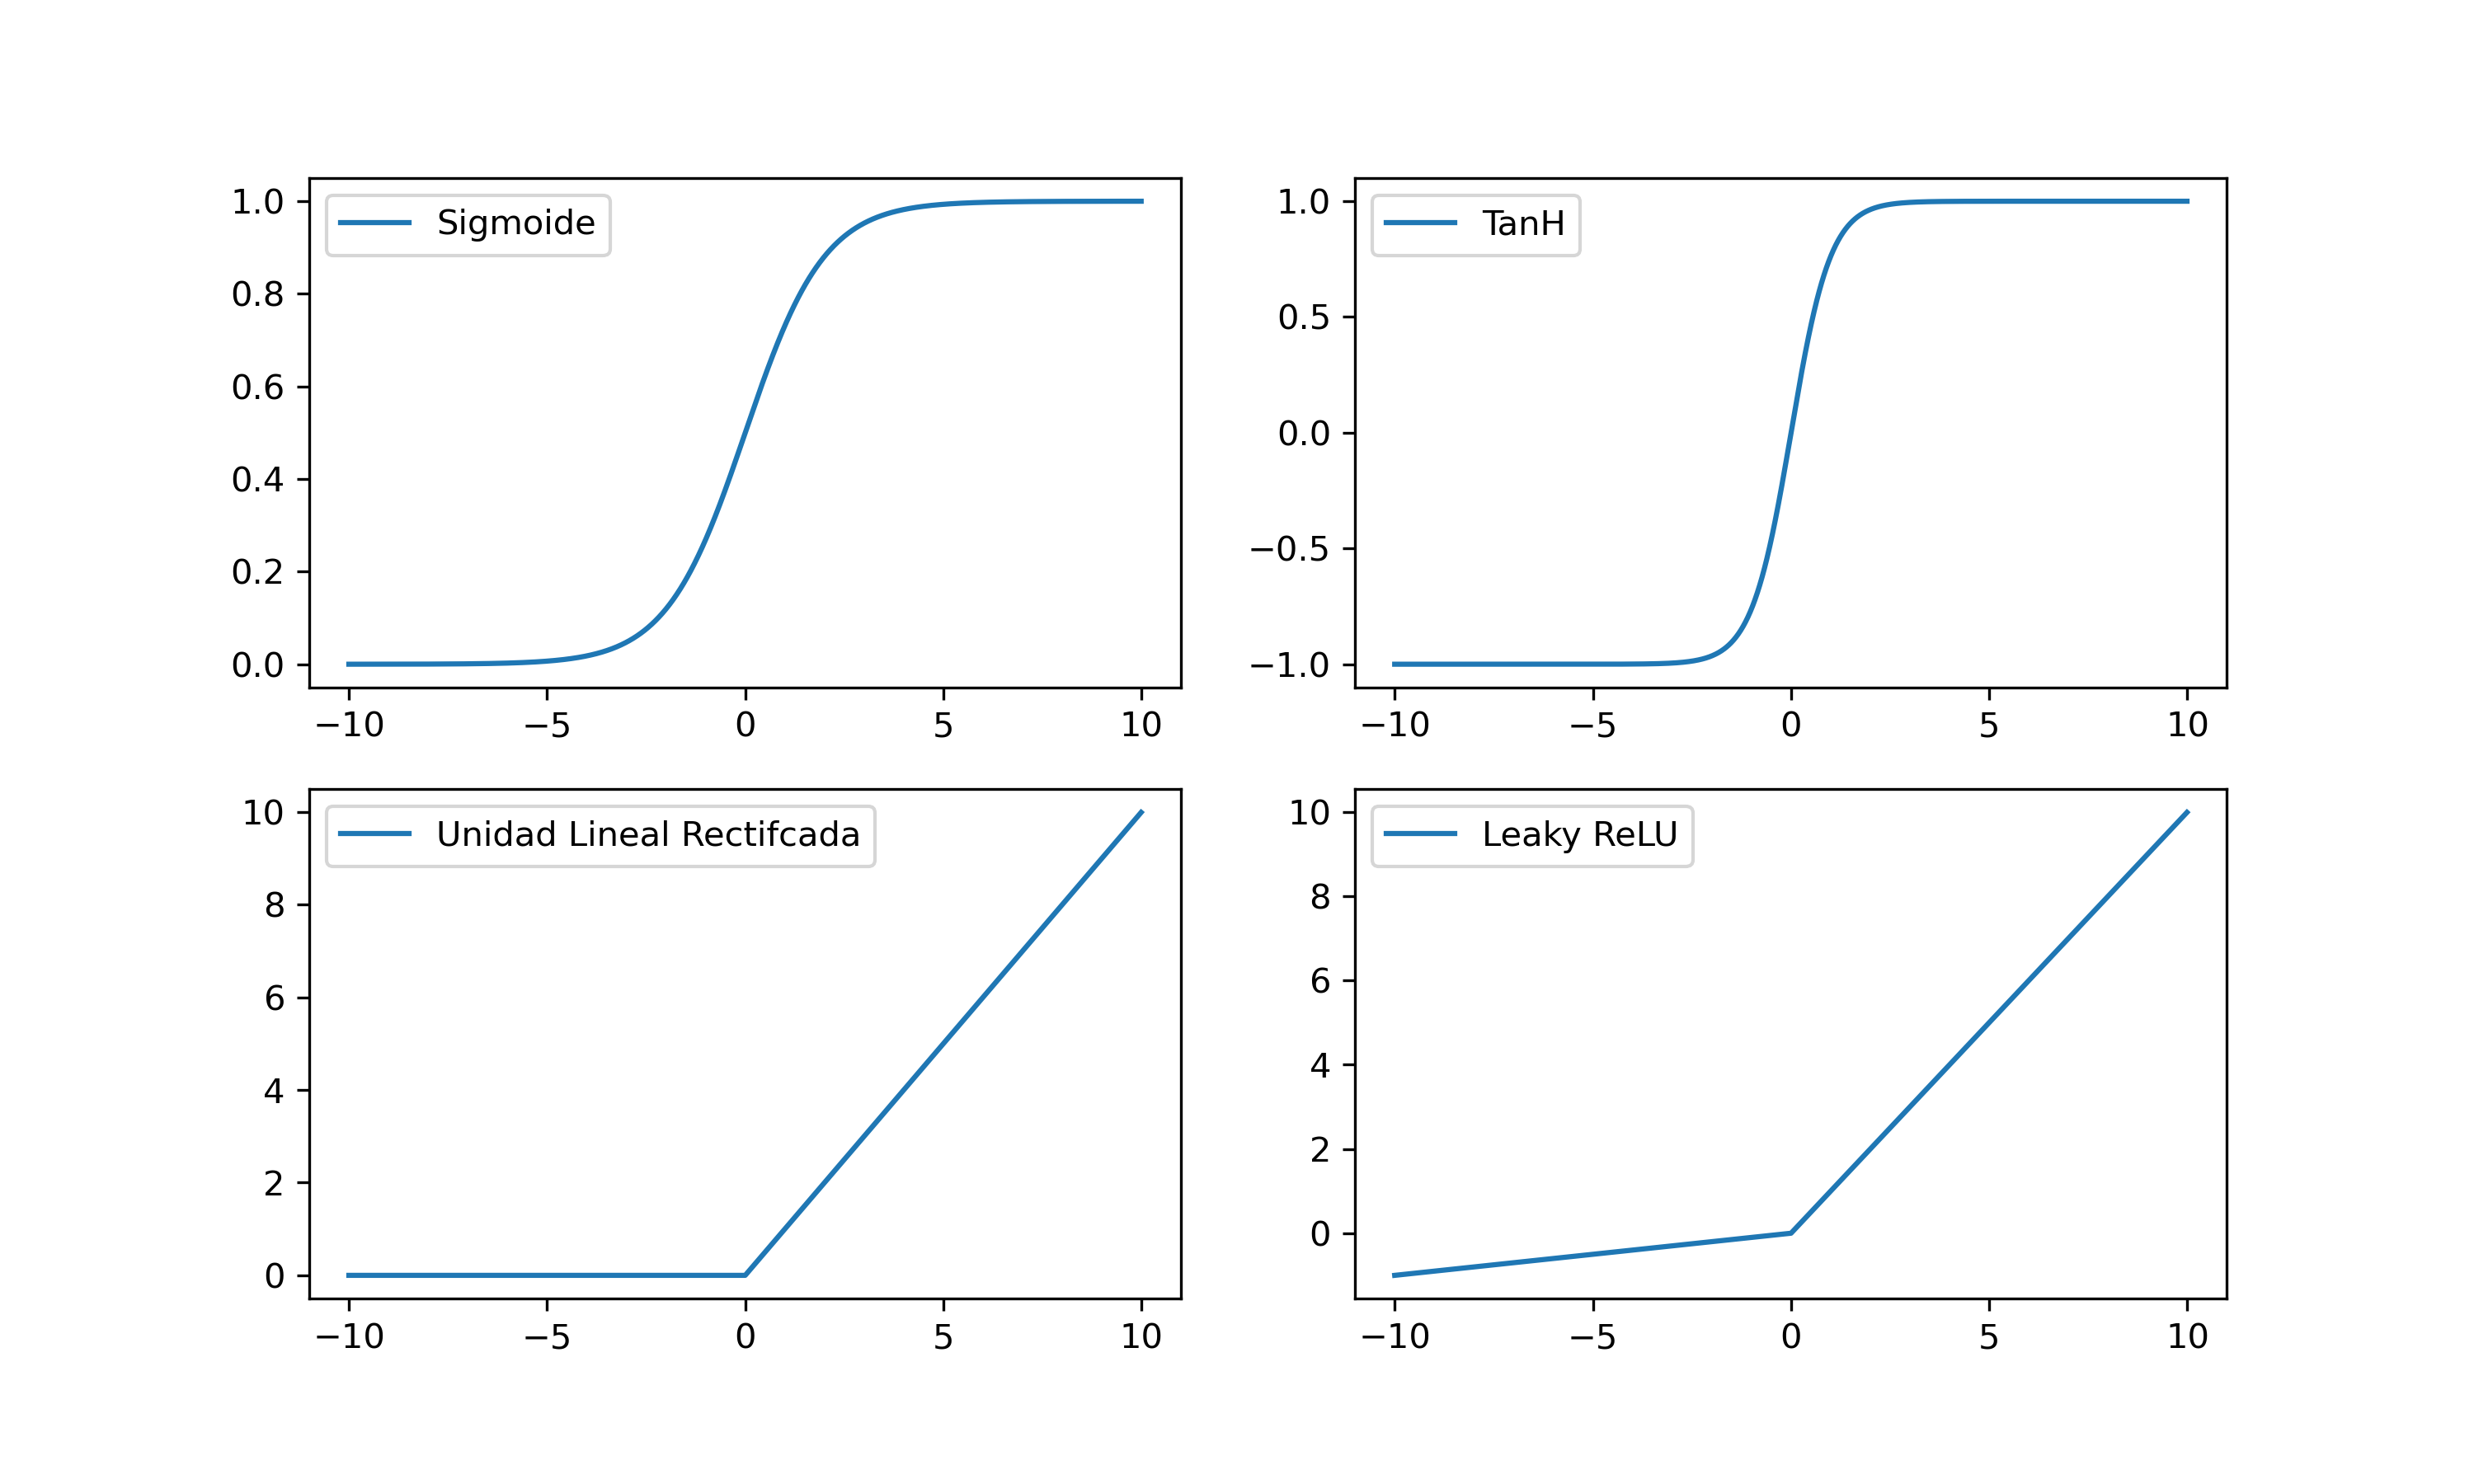
\includegraphics[width=\textwidth, keepaspectratio, height=7 cm]{images/funcionesdeactivacione.png}
            \caption{Funciones de activación}
            \label{fig:funciones de activacion}
        \end{figure}
\end{itemize}

El tipo de entrada que requiere las funciones de tensorflow/keras para el tipo
de modelo sequential, requieren un tipo de entrada numpy.array().
\begin{lstlisting}[language=Python, caption=Adecuación de los vectores de entrada usando numpy]
# 70% datos para entrenamiento, de mi dataset(datos Crudos)
## X = Matriz entrada (TA, DP) = (HR)
X_train = np.array(X_train)
## y = Salida (HR)
y_train = np.array(y_train)

# 30% datos para validacion, de mi dataset(datos Crudos)
## X = Matriz entrada (TA, DP)
X_test = np.array(X_test)
## y = Salida (HR)
y_test = np.array(y_test)

\end{lstlisting}

Finalmente para entrenar el modelo se utiliza la función model.fit(), contenida
en dentro de la clase sequential. utilizando como optimizador Adam, y metrica
de error(loss) Error Cuadrático medio.

A continuación se muestran algunos de los argumentos que requiere esta función.

\begin{itemize}\itemsep=-5px
    \item Entrada/salida(X\_train, y\_train): Estos argumentos representan en
        que variables se encuentran alojados los conjuntos que se utilizaran
        para entrenar los modelos. en este caso model2.
    \item Validation\_data: Sirve para representar la capacidad del modelo para
        estimar datos, siendo este un conjunto de datos externo a los datos de
        entrenamiento del modelo.
    \item Batch\_size: Representa la cantidad de muestras de los datos a cargar
        por etapa de entrenamiento.
\end{itemize}
\begin{lstlisting}[language=Python, caption=Funcion para entramiento]
model2.compile(optimizer=Adam(0.0001), loss='mse')
r = model2.fit(X_train, y_train,
              validation_data=(X_test,y_test),
              batch_size=16,
              epochs=800)
\end{lstlisting}
\subsection{Análisis de resultados para distintos casos y arquitecturas}

Métricas de evaluación usadas para la revisión de los modelos, a continuación
se describen algunas de las medidas mas comunes. 

\textbf{Simbolos}:  
\begin{itemize}
    \item{\textbf{$y_i$}: Resultado real esperado}
    \item{\textbf{$\hat{y}_i$}: Predicción del modelo}
    \item{\textbf{$n$}: Tamaño de la muestra}
\end{itemize}
Error absoluto medio (MAE): Es la media del error absoluto 
\begin{equation*}
    \frac 1n\sum_{i=1}^n|y_i-\hat{y}_i|
\end{equation*}

Error Cuadrático medio (MSE) Este es el promedio de los errores cuadráticos
medios

\begin{equation*}
    \frac 1n\sum_{i=1}^n(y_i-\hat{y}_i)^2
\end{equation*}
\begin{itemize}
    \item Ventajas 

        Útil si se tienen valores inesperados, que nos deberian interesar, muy
        alto o bajo valor que debemos prestar atencion.

    \item Desventajas 

        Si hacemos un predición muy mala, la cuadratura empeorara aun mas el
        error y puede sesgar la metrica para sobreestimar la maldad del modelo.
        Este es un compartamiento particularmente problemático si tenemos datos
        ruidosos. 

\end{itemize}

Raíz del error cuadrático medio (RMSE) Es la raíz cuadrado de la media del
error de cuadrados:
\begin{equation*}
    \sqrt{\frac 1n\sum_{i=1}^n(y_i-\hat{y}_i)^2}
\end{equation*}

Características generales de los errores. 

\textbf{MAE} Este es el mas sencillo de entender, siendo este el promedio el
error en la muestra. 

\textbf{MSE} Este tiene características similares al MAE, sin embargo este
tiende a disminuir los errores largos, que terminan siendo inútiles en
aplicaciones reales. 

\textbf{RMSE} Este es útil dado que los valores se pueden interpretar en
función de la salida.

Todos estos sirven para entrenar a una red neuronal, serian las funciones de
perdida que buscamos minimizar, haciendo uso de los distintos algoritmos de
optimización, en este caso estamos haciendo uso en la mayor parte del
optimizador Adam.

Para calcular esto errores se tiene las siguiente funciones en python. 
\begin{lstlisting}[language=Python, label=f_eval, caption= definicion de
funciones de evaluacion utilizando sklearn como herramienta base]
#Librerias
from sklearn import metrics
from sklearn.model_selection import cross_val_score
#Funcion de evaluacion para imprimir en la consola.
def print_evaluate(true, predicted):  
    mae = metrics.mean_absolute_error(true, predicted)
    mse = metrics.mean_squared_error(true, predicted)
    rmse = np.sqrt(metrics.mean_squared_error(true, predicted))
    r2_square = metrics.r2_score(true, predicted)
    print('MAE:', mae)
    print('MSE:', mse)
    print('RMSE:', rmse)
    print('R2 Square', r2_square)
    print('__________________________________')
'''
Funcion de evaluacion que devuelve variables, para ser usadas en alguna otra
funcion.ej. para crear una data frame en pandas con las metricas de evaluacion. 
'''
def evaluate(true, predicted):
    mae = metrics.mean_absolute_error(true, predicted)
    mse = metrics.mean_squared_error(true, predicted)
    rmse = np.sqrt(metrics.mean_squared_error(true, predicted))
    r2_square = metrics.r2_score(true, predicted)
    return mae, mse, rmse, r2_square
\end{lstlisting}

Haciendo uso de las funciones del código \ref{f_eval}, se evalúan los modelos
ya entrenados. Con dos  salida posibles por la salida estándar en tipo crudo, y
en formato de salida de pandas.

\begin{lstlisting}[language=Python, caption=Funciones  utilizadas en la
evaluación de los modelos]
# stdout
test_pred = model2.predict(X_test)
train_pred = model2.predict(X_train)
print('Test set evaluation:\n_____________________________________')
print_evaluate(y_test, test_pred)
print('Train set evaluation:\n_____________________________________')
print_evaluate(y_train, train_pred)
# dataframe de resultados
results_df = pd.DataFrame(data=[["NN para UAS 2019-2020", *evaluate(y_test, test_pred)]],columns=['Model', 'MAE', 'MSE', 'RMSE', 'R2 Square'])
results_df
\end{lstlisting}
\begin{table}[H]
    \centering
    \begin{tabular}{|p{5cm}|p{2cm}|p{2cm}|p{2cm}|p{2cm}|}\hline
        Modelo & MAE	& MSE	&RMSE	&R2 Square\\\hline
        NN para UAS 2019-2020 & 5.680064 & 43.625018 & 6.604924	& -1.575113\\
        \hline
    \end{tabular}
    \caption{Salida(tipo dataframe) para el modelo entrenado para los datos uas
    2019-2020}
    \label{model1}
\end{table}

El cuadro \ref{model1}, corresponde a una arquitectura  de capa interconectada
completamente o también llamada de capas densas:
[2,dropout(0.2),64,dropout(0.2),128,dropout(0.2),32,dropout(0.2),1]; usando
como algoritmo de optimización Adam, y un tamaño de batch = 16, con un total de
800 épocas(veces que se repite el proceso de entrenamiento).

Análisis de los resultados usando un gráfico de dispersión, de los valores
reales contra los valores predichos por dichos modelos. 

\begin{figure}[H]
    \centering
    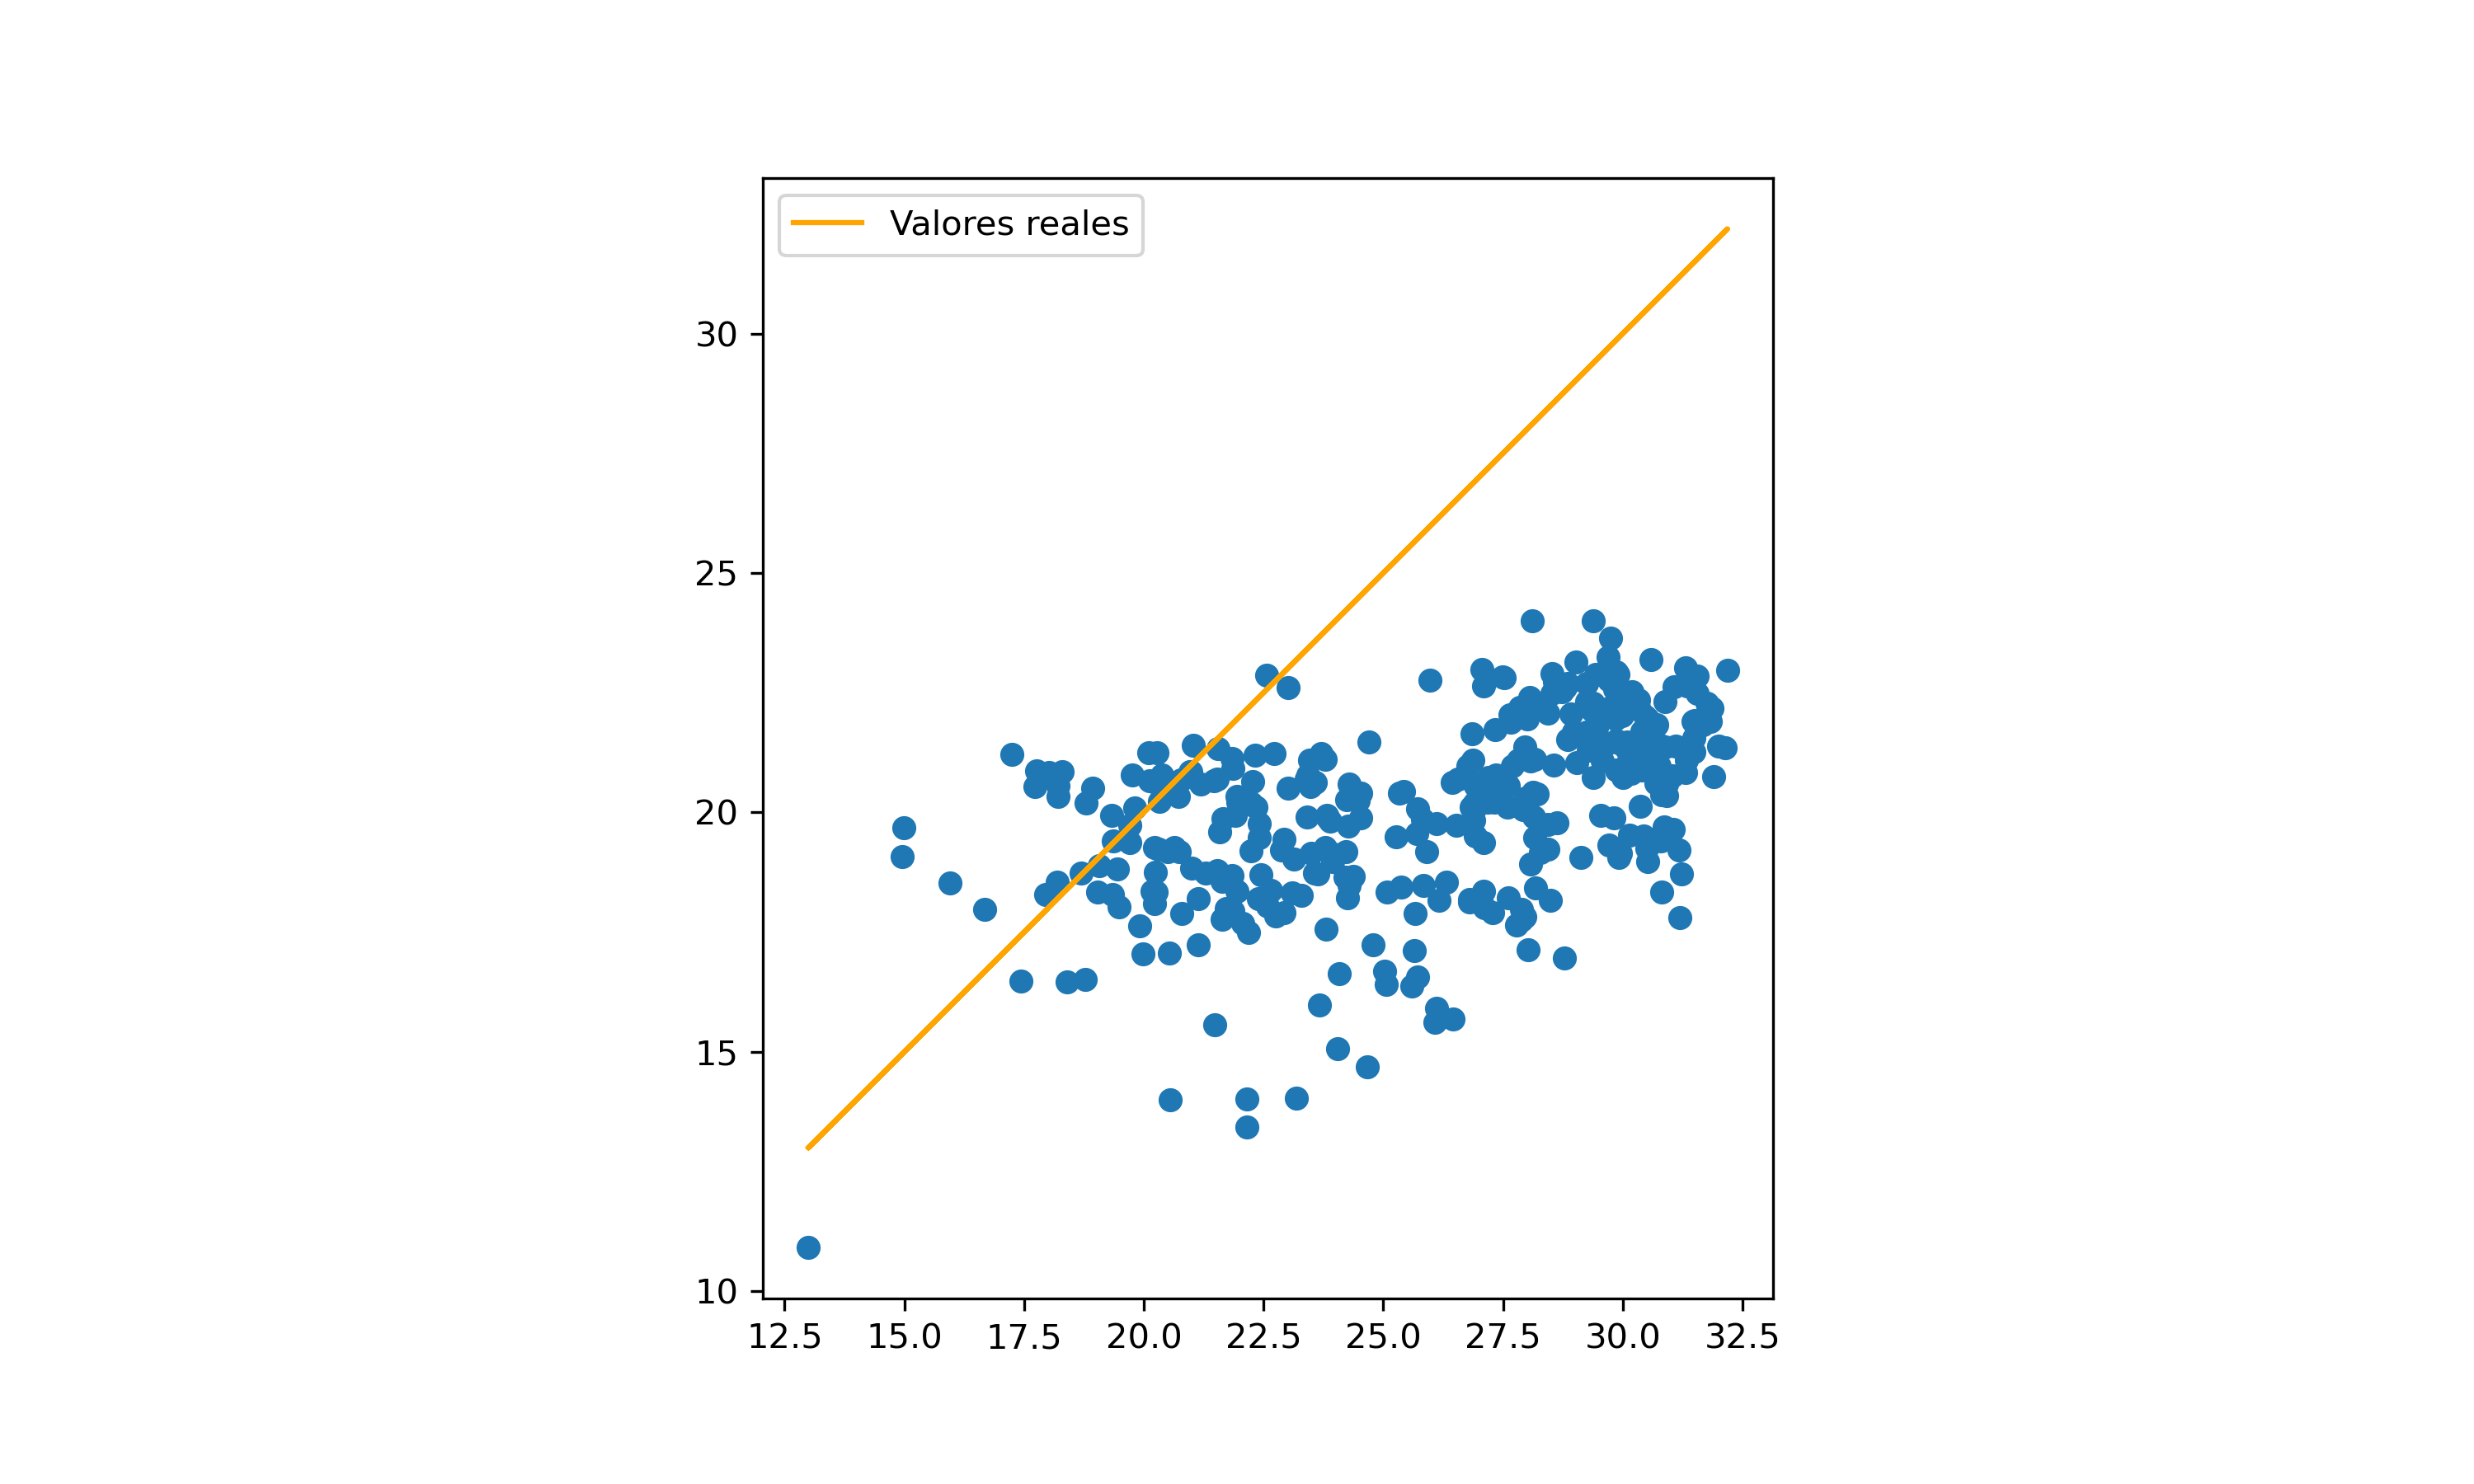
\includegraphics[width=\textwidth, keepaspectratio,
    height=7cm]{images/resultados-modelo1-dispersion.png}
    \caption{Gráfico de dispersión del modelo "NN para UAS 2019-2020"}
    \label{fig:dispersion-resultados-uas}
\end{figure}


\begin{lstlisting}[language=Python, caption=]

\end{lstlisting}

\begin{lstlisting}[language=Python, caption=]

\end{lstlisting}
\begin{lstlisting}[language=Python, caption=]

\end{lstlisting}
\begin{lstlisting}[language=Python, caption=]

\end{lstlisting}
\begin{lstlisting}[language=Python, caption=]

\end{lstlisting}
\begin{lstlisting}[language=Python, caption=]

\end{lstlisting}

%%%%%%%%%%%%%%%%%%%%%%%%%%%%%%%%%%%%%%%%%%%%%%%%%%%%%%%%%%%%%%%%%%%%%%%%%%
\subsection{Configuraciones del monitor}
La arquitectura usada para la telemetría se encuentra definida en la figura
\ref{fig:arquitectura_general_monitor}

\begin{figure}[H]
    \centering
    \includesvg[width=\linewidth,
    inkscapelatex=false]{images/arquitectura_telemetria.svg}
    \caption{Arquitectura general}
    \label{fig:arquitectura_general_monitor}
\end{figure}


Durante la configuración de la arquitectura se hace uso de herramientas tales
como docker, docker-compose en entornos linux, usando instancias en la nube. 

\newpage
\subsubsection{Configuración MQTT broker}

\begin{flushleft}
  \textbf{Configuración del servicio: MQTT broker.}
\end{flushleft}

\begin{minted}{yaml}
  mosquitto: 
    image: eclipse-mosquitto:2 
    ports:
      - 1883:1883 
    volumes:
      - ./mosquitto/mosquitto.conf:/mosquitto/config/mosquitto.conf 
      - mosquitto_data:/mosquitto/data 
      - mosquitto_log:/mosquitto/log 
\end{minted}

En esta sección se definen las siguientes propiedades. 
\begin{enumerate}
  \item Nombre del servicio dentro del archivo docker-compose.yml.
  \item Vamos a utilizar la versión 2 de la imagen oficial eclipse-mosquitto.
  \item El broker MQTT estará aceptando peticiones en el puerto 1883.
  \item Creamos un volumen de tipo bind mount para enlazar el archivo de
    configuración mosquitto.conf que tenemos en nuestro directorio local
    mosquitto con el directorio /mosquitto/config/mosquitto.conf del broker
    MQTT.
  \item Creamos un volumen para almacenar los mensajes que se reciben.
  \item Creamos un volumen para almacenar los mensajes de log.
\end{enumerate}

Es necesario realizar una configuración dentro del archivo
./mosquitto/mosquitto.conf para poder admitir conexiones al broker. 
\begin{minted}{yaml}
listener 1883
allow_anonymous true
\end{minted}
Donde se indica lo siguiente: 
\begin{enumerate}
  \item{listener 1883: es para habilitar la interfaz y el puerto en escucha del
    borker}
  \item{allow\_anonymous: deshabilita los protocolos de autenticación. siendo
    necesario indicarlo en algunas versiones del broker. }
\end{enumerate}

\begin{flushleft}
  \textbf{Configuración del servicio: Telegraf}
\end{flushleft}
\begin{minted}{yaml}
  telegraf: 
    image: telegraf:1.18 
      volumes:
        - ./telegraf/telegraf.conf:/etc/telegraf/telegraf.conf 
      depends_on: 
        - influxdb
\end{minted}
\begin{enumerate}
  \item Nombre del servicio dentro del archivo docker-compose.yml.
  \item Utilizamos la imagen Docker telegraf que tiene la etiqueta 1.18.
  \item Creamos un volumen de tipo bind mount para enlazar el archivo de
    configuración telegraf.conf que tenemos en nuestro directorio local
    telegraf con el archivo /etc/telegraf/telegraf.conf del contenedor.
  \item Indicamos que este servicio depende del servicio influxdb y que no
    podrá iniciarse hasta que el servicio de influxdb se haya iniciado.
\end{enumerate}

A partir de crear el servicio, es necesario genera un archivo de configuración, 
\begin{minted}{bash}
docker run --rm telegraf telegraf config > telegraf.conf
\end{minted}
Una vez creado el archivo es de configuración es necesario alojarlo en como se
muestra a continuación. (./telegraf/telegraf.conf)
\begin{minted}{bash}
.(directorio base)
--docker-compose.yml
----mosquitto
     --mosquitto.conf
----telegraf
     --telegraf.conf
\end{minted}
Dentro del mismo se encuentran bastantes configuraciones, disponibles para todos
los servicios y protocolos que soporta telegraf, sin embargo para el propósito
de la aplicación solo es necesario configurar las siguientes secciones.

\begin{enumerate}
  \item inputs.mqtt\_consumer: En este se encuentran definidas todas las
    propiedades y configuraciones requeridas para realizar la conexion hacia el
    broker MQTT en este caso mosquitto-eclipse. 
  \item output.influxdb: Aloja las configuración relacionadas a la salida que e
    este generara.
\end{enumerate}

Para el caso de inputs.mqtt\_consumer, hay distintos parametros de
configuración.
\begin{enumerate}
  \item servers:En este es necesario indicar la url donde esta alojado el
    broker, para este proyecto dado que se esta haciendo uso de docker solo es
    necesario poner el nombre del servicio. 
  \item topics: indica los tópicos a los que el cliente(telegraf) se
    subscribirá. 
  \item data\_format: indica el formato del tipo de dato que estaremos
    recibiendo a travez del mqtt broker. 
\end{enumerate}
\begin{minted}{bash}
 [[inputs.mqtt_consumer]]
   servers = ["tcp://mosquitto:1883"] 

   topics = [
     "esp23/#" //indica que nos queremos subscribir  a todos los topics a
     //partir de esp32
   ]

   data_format = "influx" 
\end{minted}

Por otro lado, para el caso de output.influxdb, los parametros son los
siguientes:
\begin{enumerate}
  \item Urls: indica el url de donde esta alojada el servicio de influxdb,
    (igual que el caso anterior el url corresponde con el nombre del servicio
    en docker)
  \item Database: indica el nombre de la base de datos. 
  \item Skip\_database\_creation: valor booleano que define si se crearan o no,
    las bases de datos, generalmente la idea es tener la tabla definida con
    anterioridad. 
  \item Username: corresponde a los nombres de usuario declarados en el
    servicio de docker-compose. 
  \item Password:corresponde a las contraseñas declaradas en el
    servicio dentro del archivo docker-compose.yaml.
\end{enumerate}



\begin{flushleft}
  \textbf{Configuración del servicio: InfluxDB}
\end{flushleft}

\begin{minted}{yaml}
influxdb: 
    image: influxdb:1.8 
    ports:
      - 8086:8086 
    volumes:
      - influxdb_data:/var/lib/influxdb 
    environment:
      - INFLUXDB_DB=esp32 
      - INFLUXDB_ADMIN_USER=root 
      - INFLUXDB_ADMIN_PASSWORD=root 
      - INFLUXDB_HTTP_AUTH_ENABLED=true 
\end{minted}

\begin{enumerate}
  \item Nombre del servicio dentro del archivo docker-compose.yml.
  \item Utilizamos la imagen Docker influxdb que tiene la etiqueta 1.8.
  \item Este servicio utilizará el puerto 8086 de nuestra máquina local para
    enlazarlo con el puerto 8086 el contenedor.
  \item Creamos un volumen con el nombre influxdb\_data que estará enlazado con
    el directorio /var/lib/influxdb del contenedor.
  \item Nombre de la base de datos.
  \item Usuario de la base de datos.
  \item Contraseña del usuario de la base de datos.
  \item Habilitamos la autenticación básica HTTP.
\end{enumerate}

\begin{flushleft}
  \textbf{Configuración del servicio: Grafana}
\end{flushleft}
La configuración de grafana esta conpuesta con las siguientes bases.

\begin{minted}{yaml}
grafana: 
    image: grafana/grafana:7.4.0 
    ports:
      - 3000:3000 
    volumes:
      - grafana_data:/var/lib/grafana 
      - ./grafana-provisioning/:/etc/grafana/provisioning 
    depends_on: 
      - influxdb
\end{minted}

\begin{enumerate}
\item Nombre del servicio dentro del archivo docker-compose.yml.
\item Utilizamos la imagen Docker grafana.
\item Este servicio utilizará el puerto 3000 de nuestra máquina local para
  enlazarlo con el puerto 3000 el contenedor.
\item Creamos un volumen con el nombre grafana\_data que estará enlazado con el
  directorio /var/lib/grafana del contenedor.
\item Indicamos que este servicio depende del servicio influxdb y que no podrá
  iniciarse hasta que el servicio de influxdb se haya iniciado.
\end{enumerate}


Como parte importante es necesario configurar las fuentes de datos,
configuraciones generales, en este caso, se declaran a partir de archivos yml
en diferentes directorios dentro de el espacio de trabajo de grafana. 

Archivos de configuración son los siguientes:

El archivo inferior, corresponde al aprovisionamiento automatico de las fuentes
de datos, en el caso siguiente grafana cuenta con funciones directamente para
conectase a influxDB.
\begin{minted}{yaml}
apiVersion: 1
datasources:
  - name: InfluxDB
    type: influxdb
    access: proxy
    database: esp32 
    user: root 
    password: root 
    url: http://influxdb:8086 
    isDefault: true
    editable: true
\end{minted}
Parámetros: 
\begin{enumerate}
  \item Nombre de la base de datos InfluxDB
  \item Nombre de usuario para acceder a la base de datos
  \item Contraseña del usuario para acceder a la base de datos
  \item URL del servicio InfluxDB
\end{enumerate}

El archivo de configuración inferior, crea un aprovisionamiento automático de
dashboards, donde los mismos podrían ser definidos, base a la documentación de
grafana, revisando cada uno de los parámetros que se pueden agregar al
archivo.json del dashboard a crear.
    


\begin{minted}{yaml}
apiVersion: 1
providers:
- name: InfluxDB
  folder: ''
  type: file
  disableDeletion: false
  editable: true
  options:
    path: /etc/grafana/provisioning/dashboards
\end{minted}

Parámetros: 
\begin{enumerate}
  \item Nombre del servicio dentro del archivo docker-compose.yml.
  \item Utilizamos la imagen Docker grafana.
  \item Este servicio utilizará el puerto 3000 de nuestra máquina local para
    enlazarlo con el puerto 3000 el contenedor.
  \item Creamos un volumen con el nombre grafana\_data que estará enlazado con
    el directorio /var/lib/grafana del contenedor.
  \item Creamos un volumen de tipo bind mount entre el directorio local de
    nuestra máquina ./grafana-provisioning/ y el directorio
    /etc/grafana/provisioning del contenedor.
  \item Indicamos que este servicio depende del servicio influxdb y que no
    podrá iniciarse hasta que el servicio de influxdb se haya iniciado.
\end{enumerate}


A cada archivo le corresponde un sitio en el espacio de trabajo(directorio) 

\begin{minted}{yaml}
.(directorio de trabajo)
grafana-provisioning
---dashboards
  ----CO2Dashboard.json
  ----dashboard.yml
---datasources
  ----datasource.yml
\end{minted}

En la documentación ofical se pueden obtener datos o propiedades de una
dashboard por ejemplo.
\href{https://grafana.com/docs/grafana/latest/dashboards/}{grafana
docs}.



\subsubsection{Configuración general}
Durante la configuración de los servicios y instacias requeridas se parte de
los siguietes requerimientos. 
\begin{enumerate}
  \item Docker, docker-compose. \href{https://docs.docker.com/compose/}{guia}.
  \item alguna maquina, o instancia en la nube disponible para hostear los
    servicios.
\end{enumerate}

Partiendo de ello, se llevan es necesario, seguir todas las instrucciones
anteriores para poder implementar dicho monitor. 

En la parte superior se encuentra disponible el archivo docker-compose.yml.
\begin{minted}{yaml}
version: '3'

services:
  mosquitto:
    image: eclipse-mosquitto:2
    ports:
      - 1883:1883
    volumes:
      - ./mosquitto/mosquitto.conf:/mosquitto/config/mosquitto.conf
      - mosquitto_data:/mosquitto/data
      - mosquitto_log:/mosquitto/log

  telegraf:
    image: telegraf:1.18
    volumes:
      - ./telegraf/telegraf.conf:/etc/telegraf/telegraf.conf
    depends_on:
      - influxdb

  influxdb:
    image: influxdb:1.8
    ports:
      - 8086:8086
    volumes:
      - influxdb_data:/var/lib/influxdb
    environment:
      - INFLUXDB_DB=${INFLUXDB_DB}
      - INFLUXDB_ADMIN_USER=${INFLUXDB_USERNAME}
      - INFLUXDB_ADMIN_PASSWORD=${INFLUXDB_PASSWORD}
      - INFLUXDB_HTTP_AUTH_ENABLED=true

  grafana:
    image: grafana/grafana:7.4.0
    ports:
      - 3000:3000
    volumes:
      - grafana_data:/var/lib/grafana
      - ./grafana-provisioning/:/etc/grafana/provisioning
    depends_on:
      - influxdb

  chronograf:
    image: chronograf:1.8
    ports:
      - 8888:8888
    volumes:
      - chronograf_data:/var/lib/chronograf
    depends_on:
      - influxdb
    environment:
      - INFLUXDB_URL=http://influxdb:8086
      - INFLUXDB_USERNAME=${INFLUXDB_USERNAME}
      - INFLUXDB_PASSWORD=${INFLUXDB_PASSWORD}

volumes:
  mosquitto_data:
  mosquitto_log:
  node_red_user_data:
  influxdb_data:
  grafana_data:
  chronograf_data:
\end{minted}

Finalmente seria tan simple como usar el comando docker-compose up -d para
correr todos los servicios que involucran a la solucion, y declarar un par
variables de entorno (.env), serian las contraseñasde influxdb, usuario, nombre
de la base de datos, y las credenciales para grafana. todas estas se ecunetran
entre llave, con un signo de dolar al inicio dentro del archivo de
configuración.

\textbf{**Nota:} En el caso del proyecto en mencion se esta haciendo uso del
servicio ec2 de Amazon Web Services, para alojar la maquina virtual que soporta
los servicios. Siendo posible instanciar dichos servicios en un entorno local
con ciertas características**.

{\tiny ** una ip publica, en caso de no estar alojada esta en la misa seccion
de red.}




%%%%%%%%%%%%%%%%%%%%%%%%%%%%%%%%%%%%%%%%%%%%%%%%%%%%%%%%%%%%%%%%%%%%%%%%%%
\section{Referencias} 
\bibliographystyle{IEEEtran} 
\bibliography{refer}
\section{Anexos} 
\subsection{Cronograma}
    
\begin{table}[H]
  \centering
  \resizebox{\textwidth}{!}{%
    \begin{tabular}{{p{10cm}}*{16}{m{0.2cm}}}\hline
      &\multicolumn{16}{c}{Semanas}\\\cmidrule{2-17}
      Actividad & 1& 2& 3& 4& 5& 6& 7& 8& 9& 10& 11& 12& 13& 14& 15& 16\\\hline
      Análisis de los requerimientos del proyecto y estudio de los recursos
      que se tiene para su desarrollo.
      &  x&  x&  x& & & & & & & & & & & & & \\\midrule
      Realizar el acondicionamiento del sistema de humedad de suelo en el
      micro-invernadero, con el fin de tener las condiciones adecuadas para la
      captura de datos reales del sistema para el diseño del modelo por redes
      neuronales.\vspace{2mm}  Desarrollar los temas relacionados al modelado en sistemas
      de tipo invernadero. A su vez se comenzará a evaluar la integridad del
      cronograma propuesto, y estructuración del informe final, buscando
      realizar las primeras revisiones de estos (informe y cronograma).
      & & & & x& x& & & & & & & & & & & \\\midrule
      Durante estas semanas comenzaremos a documentar características que
      definen a los sistemas de redes neuronales el resultado esperado de las
      primeras semanas (4,5,6,7,8), corresponde a localizar características,
      ventajas, conceptos prácticos aplicables, detección de entradas y
      salidas, a controlar dentro del sistema invernadero.  Partiendo de la
      documentación revisada, procedo a diseñar un modelo de redes neuronales
      utilizando estructuras conocidas (MLP modelo de perceptrón multicapas o
      modelos de capas densas) que representen al sistema físico, empleando las
      tecnologías que se localicen durante la investigación relacionadas al
      campo de inteligencia artificial, con anterioridad se han estado
      revisando distintas herramientas tales como Simulink (empleando toolkits
      para modelar rápidamente), herramientas enfocadas ( keras, tensorflow,
      pytorch) muchas de estas empleadas en los campos de IA con un gran
      impacto en la actualidad. \vspace{2mm}

      A partir del diseño a presentar. Lo siguiente
      seria simular los modelos de redes neuronales, validando así los mimos.
      Con el fin de estudiar y verificar toda la información obtenida, durante
      el proceso anterior.
      & & & & x& x& x& x& x& x& x& x& x& & & &\\\midrule
      Se finalizará el proceso de escritura del informe final para su entrega.
      & & & & & & & & & & & & & x& x& x& x\\\hline
  \end{tabular}}
  \caption{Cronograma de actividades esperado}
  \label{t:cronograma}
\end{table}

\textbf{Nota: }Durante el periodo de residencias ago.-dic. 2021, se busca estar revisando de
manera periódica (cada mes), el informe final, mismo que tiene como finalidad
ser la introducción a mi proyecto de tesis.

\end{document}
